\cleardoublepage

\chapter{Dream content}
\label{sec:dream-content}

\cleanchapterquote{Prétendre donner les rêves comme de simples jeux de la pensée, de simples images de l’imagination, c’est témoigner d’un manque de réflexion ou de loyauté ; car de toute évidence ils en diffèrent spécifiquement. Les images de l’imagination sont faibles, languissantes, incomplètes, partielles et si fugitives qu’on peut à peine fixer dans sa mémoire pendant quelques secondes les traits d’un absent, et que même le jeu le plus vif de l’imagination ne peut nullement entrer en comparaison avec la réalité palpable que le rêve met sous nos yeux.}{Schopenhauer}{Parerga und Paralipomena, 1851}

\section{Basic principles of dream content analysis}
\label{sec:dream-content:method}

Empirical investigation on dreaming started in the nineteenth century when amateur researchers started to quantify aspects of their dream content. One notable example is the pioneering paper of Mary Calkins \citeyearpar{calkins_statistics_1893}, entitled \q{Statistics of dreams}, in which she reported, inter alia, statistics concerning dream length and vividness, dream characters and dream- and waking-life associations. Since then, a considerable numbers of scales and rating systems for dream content analysis have been developed \citep{schredl_dream_2010}. Most of them are based on automatic analysis of the lexical content of dream reports, a method which has the advantages of minimizing the experimenter bias and being replicable by other research groups. Perhaps the most famous is the Hall \& Van de Castle system, which have provided a global profile of dream content dimensions in young adult \citep{hall_content_1966}. It remains today the major reference since it has proven stable over at least one generation \citep{hall_dreams_1982}.

\section{Quantitative results}
\label{sec:dream-content:quant}

Results from several decades of dream content studies \citep{hall_content_1966, schwartz_exploration_1999, schredl_characteristics_2010} indicate that: dreams tend to be negative on many dimensions and aggressions are more frequent than friendly interactions, visual imagery occurs more frequently in dreams than imagery of other senses (audition, olfaction, touch, and taste); the dream drama is mostly lived by the dreamer from a first-person perspective; some elements of real-life events previously experienced by the dreamer often contribute to the scene of the dream; most often, the dream sequence is not within the dreamer’s voluntary control (i.e., the dreamer may be convinced during the dream that the dream’s story is really happening); temporal and spatial incoherencies can occur in the dream story; the dream report is often full of people interacting with each other (e.g., discussions, fights, pursuit, sexuality); and finally, the dream report often contains strong emotions.
Gender differences in dream content have been consistently reported. For example, men report more often physical aggression and sex than women \citep{nielsen_typical_2003, schredl_typical_2004}.
Finally, many aspects of the subject’s daily life influence dream content (reviewed in \citealp{ruby_experimental_2011}), including news event, musical practice, current concerns and religious beliefs, chronic pain, mood or living in a violent environment.

\section{The sources of dream content}
\label{sec:dream-content:sources}

Based on these experimental findings, \citet{de_koninck_sleep_2012} has reviewed in his book entitled \q{Sleep, dreams and dreaming} the sources that mediate dream construction, as well as their relative contribution to the dream content. He proposed that the different sources of dreams are best represented in a pyramidal manner, from low, more biological levels, predominant in shaping the dream content, to higher, more cognitive levels, that carry much less influence to the dream content (Figure \ref{fig:intro:koninck}).

\begin{figure}[htb]
	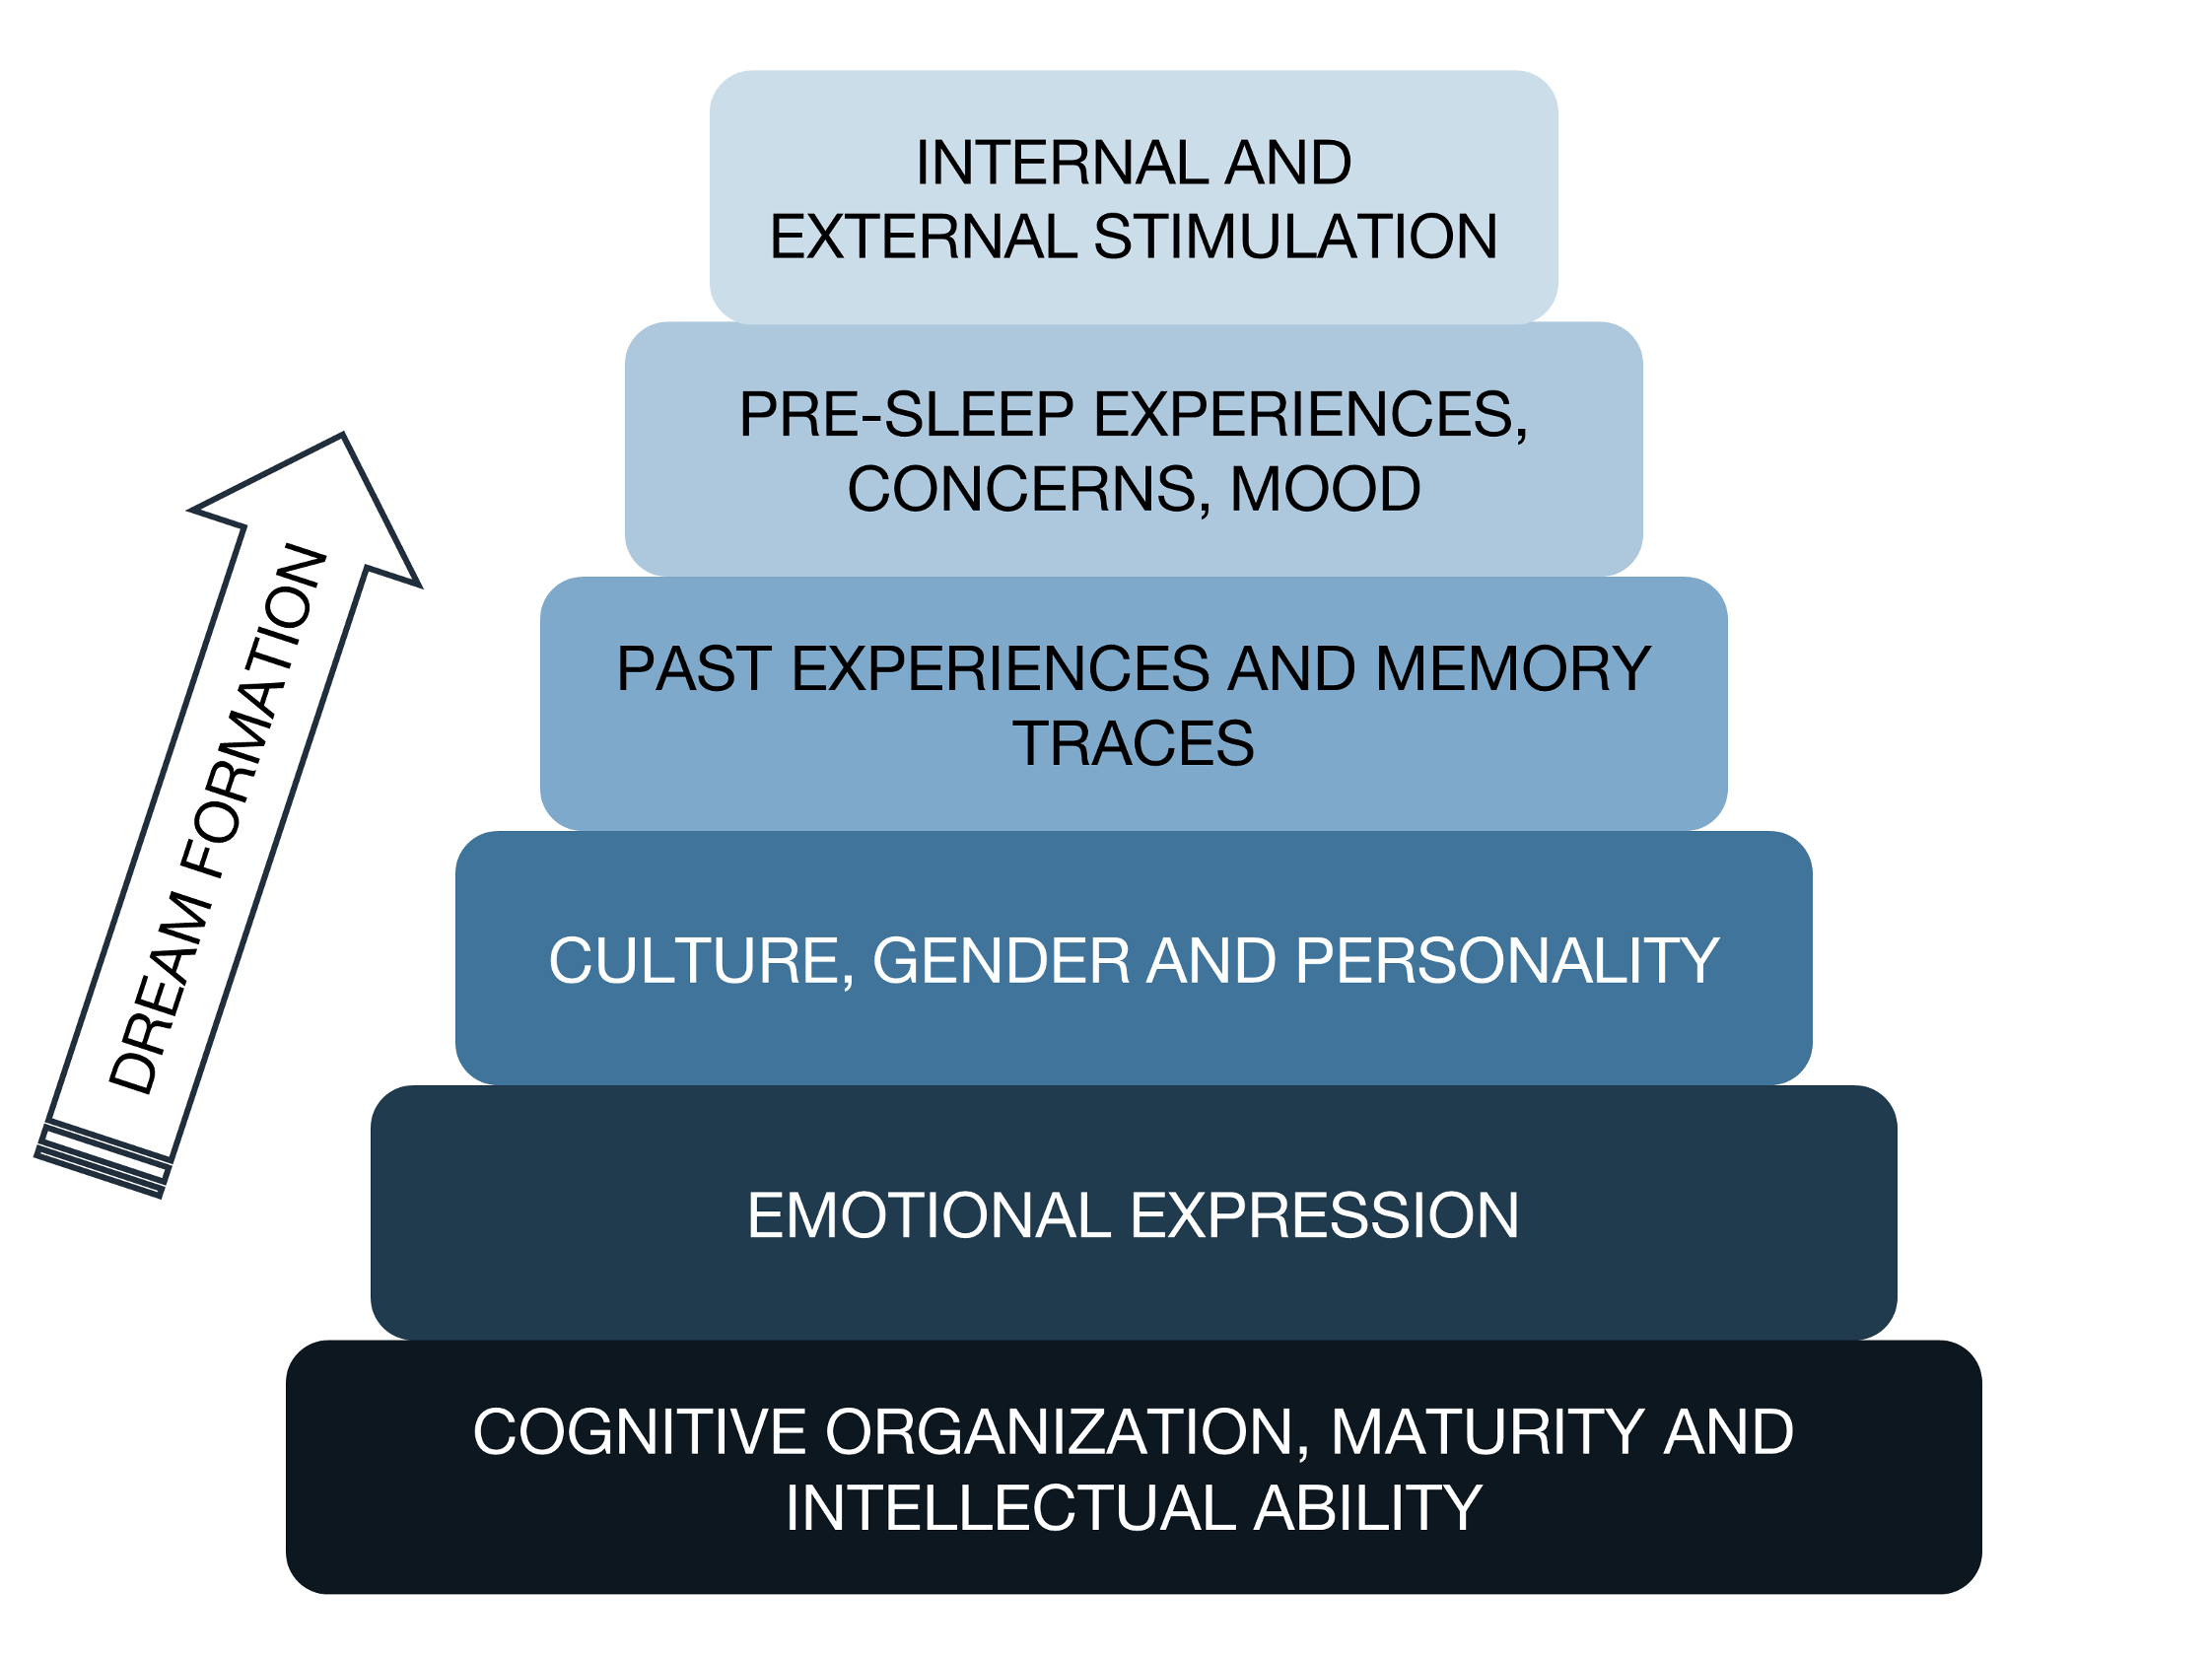
\includegraphics[width=\textwidth]{Fig/Intro/Intro_Pyramid_dream_construction/Intro_pyramid_dream.png}
	\caption[Layers in the construction of dreams]{Layers in the construction of dreams \citep{de_koninck_sleep_2012}. The various factors in the elaboration of dreaming are illustrated as a pyramid suggesting their order and importance.}
	\label{fig:intro:koninck}
\end{figure}

\subsection{The memory sources of dreams}
\label{sec:dream-content:sources:memory}

As we mentioned earlier, there is ample evidence that waking experience finds its way into dreams. However, the characteristics and time course of the waking memory sources integrated into dreams are still unclear. For instance, it is now clear that dream content very rarely replays an episodic memory as it is remembered \citep{fosse_dreaming_2003, nielsen_what_2005}, although it is often related to some elements of the waking life of the dreamer \citep{schredl_characteristics_2010, blagrove_trait_2010, ruby_experimental_2011}. This observation has led to the so-called \q{continuity hypothesis of dreaming} which simply states that dreams reflect waking life experiences \citep{schredl_continuity_2003}.

Several factors have been positively associated with the likelihood of a waking life experience to be incorporated into dreams \citep{schredl_characteristics_2010}. These factors are reviewed in the following lines. First, there seems to be a linear decrease in temporal references identified in dreams, with recent experiences being more incorporated into dreams than older ones \citep{botman_dream_1990, strauch_dem_2004, grenier_temporal_2005}. This finding supports the notion of continuity between waking and dreaming memory processes. Furthermore, several studies \citep{botman_dream_1990, nielsen_day-residue_1992, marquardt_empirical_1996} have confirmed that a significant proportion of dreams contain elements that refer to experiences of the preceding day, a phenomenon known as day-residues and mentioned by Freud who considered them as \q{a necessary ingredient in dream formation} \citep{freud_interpretation_1900}. Another interesting finding is that contrary to what would be expected according to memory decay with time, some studies reported an overrepresentation in dreams of waking experiences that happened approximately one week before the dream \citep{nielsen_day-residue_1992, marquardt_empirical_1996}, however this effect was found only for REM dreams and not N2 or N3 dreams \citep{blagrove_assessing_2011, van_rijn_dream-lag_2015}. Second, there is a preferential incorporation of emotional waking-life experiences into dreams \citep{malinowski_evidence_2014, schredl_factors_2006}. Interestingly, emotional intensity, but not emotional tone seems to affect the incorporation into subsequent dreams. Third, all waking life activities are not represented in the same proportion in dreams \citep{hartmann_we_1996, schredl_continuity_2000}. Focused thinking activity (such as using a computer, reading) are rarely reported in dreams, an effect that may be explained by the generally low emotional intensity of these types of activities. Fourth, the magnitude of the continuity between waking and dreaming is related to some extent to the personality traits of the dreamer \citep{schredl_dreaming_1996}. Finally, chronobiological factors, such as sleep cycles and time of the night, influence dream content. For example, dream reports from the first part of the night comprise more elements of the previous day than dream reports from the second part of the night \citep{roffwarg_effects_1978}.
